\documentclass[svgnames,12pt,aspectratio=149]{beamer}
\mode<presentation>%
{
  \usetheme{Boadilla}
  \setbeamercovered{dynamic}
}
\usepackage[english,spanish]{babel}
\usepackage[utf8]{inputenc}
\usepackage[T1]{fontenc}
\usepackage{sty/BeamerLille}
\usepackage{float}
\usepackage{caption}
\usepackage{subfigure} 
\usepackage{quantikz}
\usepackage{graphicx}
\graphicspath{ {./images/} }
\usepackage{tikz}


\usepackage{amssymb,amsfonts}


\title{Mediciones difusas en sistemas cuánticos\\\hspace{0.7cm}para N partículas}
\subtitle{}
\author[Rubí Ramírez] % (optional)
{Rubí Ramírez Milián}
\institute[ECFM]{
Escuela de Ciencias Físicas y Matemática\\
Universidad de San Carlos\\
\textit{Asesorado por: \\ 
Dr.\@ Carlos Pineda (IF-UNAM)}\\
Ing. Rodolfo Samayoa (ECFM-USAC)
}
\date{14 de agosto de 2024}
\AtBeginSection[]
{
 \begin{frame}
    \frametitle{Contenidos}
	\tableofcontents[currentsection]
  \end{frame}
}

\begin{document}

\begin{frame}[plain]
  \titlepage{}
\end{frame}

\begin{frame}{Agradecimientos}
     \begin{itemize}
  \item A mi familia
  \item A mis asesores
  \item A mis amigos y amigas
  \end{itemize}
\end{frame}


\section{Introducción}

\begin{frame}
  \frametitle{Motivación}

\end{frame}

\begin{frame}
  \frametitle{Introducción}


\end{frame}






\section{Revisión de literatura}
\begin{frame}
 \frametitle{Operador de densidad}
  
\end{frame}

\begin{frame}
\frametitle{Medidas POVM y operadores de Kraus}
    
\end{frame}



\section{Mediciones difusas}

\begin{frame}{Mediciones difusas}
Una medición difusa es un proceso no ideal en el cual, debido a ruido
del entorno o a fallos en el dispositivo de detección, se presenta la probabilidad de una
identificación errónea de las partículas del sistema.

\end{frame}

\begin{frame}   \begin{figure}[H]
\centering
\subfigure[]{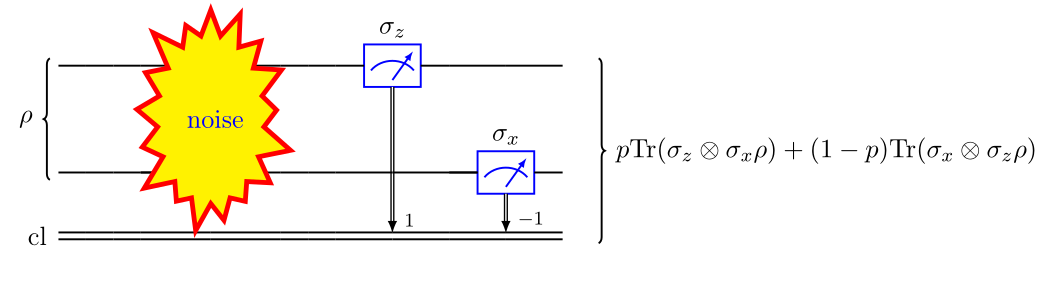
\includegraphics[width=100mm]{images/fm1.png}}
\subfigure[]{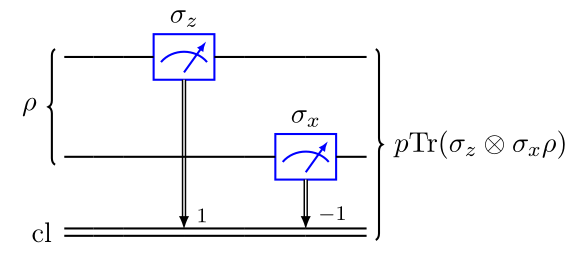
\includegraphics[width=50mm]{images/fmideal.png}}
\subfigure[]{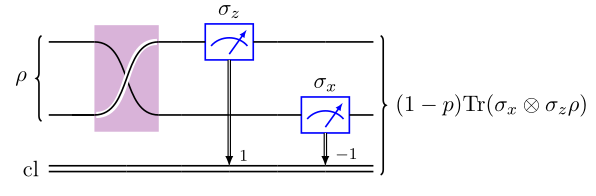
\includegraphics[width=50mm]{images/fm-nonideal.png}}

\caption{Medición difusa}\label{fig:lego}
\end{figure} 

    
\end{frame}

\begin{frame}{Valor esperado y operador difuso}
    \begin{block}{Valor esperado}
      
    \end{block}
    \begin{block}{Operador Difuso}
      
    \end{block}
\end{frame}

\begin{frame}{Instrumentos cuánticos}
    
\end{frame}


\section{Resultados}
\begin{frame}{POVM y operadores de Kraus para mediciones difusas en sistemas de dos partículas}
    
\end{frame}

\begin{frame}{Instrumentos cuánticos para dos partículas I}

\begin{figure}[H]
\centering
\subfigure[]{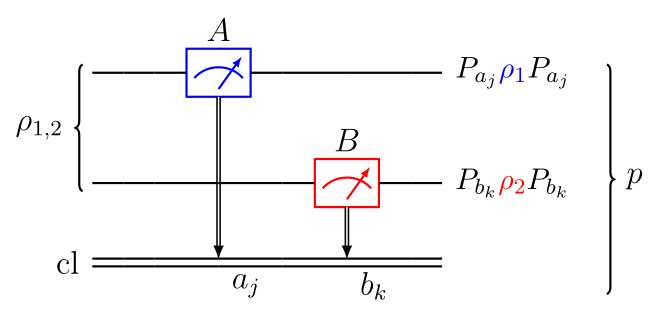
\includegraphics[width=40mm]{images/fmideaqi.png}}
\subfigure[]{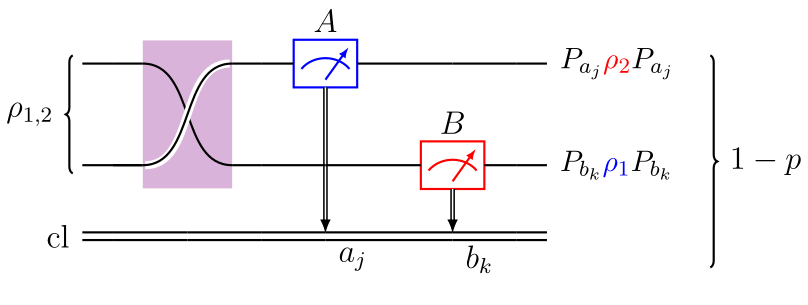
\includegraphics[width=50mm]{images/fmqi1.png}}
\caption*{}
\end{figure} 




\end{frame}

\begin{frame}{Instrumentos cuánticos para dos partículas II}
\begin{figure}[H]
\centering
\subfigure[]{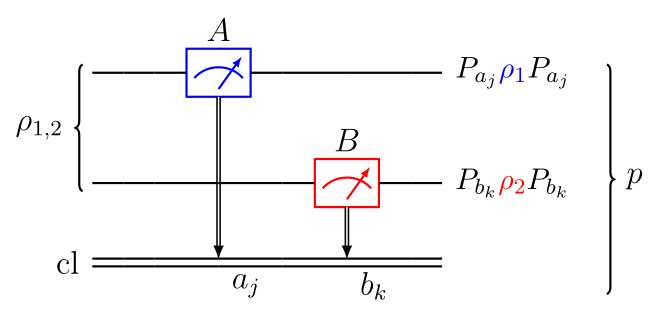
\includegraphics[width=50mm]{images/fmideaqi.png}}
\subfigure[]{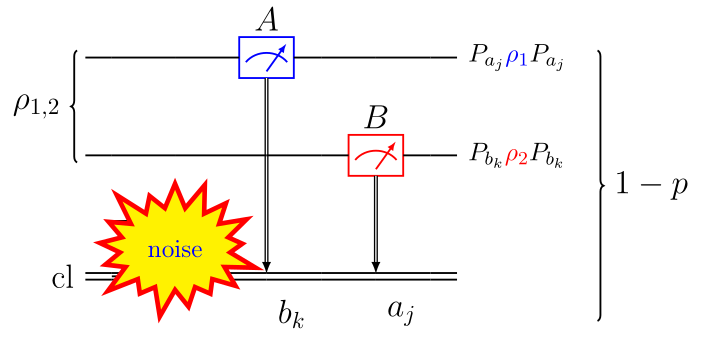
\includegraphics[width=50mm]{images/fmqi2.png}}
\caption*{} 
\end{figure} 

\end{frame}

\begin{frame}{Instrumentos cuánticos para dos partículas III}
\begin{figure}[H]
    \centering
\subfigure[]{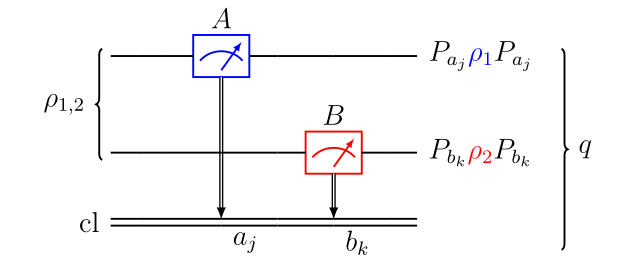
\includegraphics[width=35mm]{images/fmidealiq3.png}}
\subfigure[]{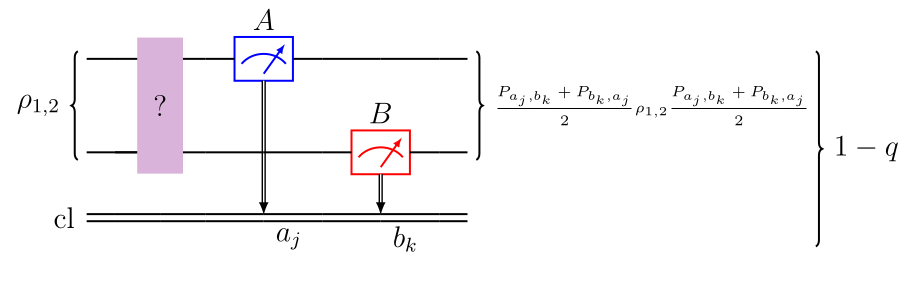
\includegraphics[width=50mm]{images/fmqi3.png}}
\caption*{} 
\end{figure} 
\end{frame}

\begin{frame}{Equivalencia}
    
\end{frame}


\begin{frame}{Generalización}
    
\end{frame}

\section{Conclusiones}

\begin{frame}{Conclusiones}
    
\end{frame}




\end{document}

%%% Local Variables:
%%% mode: latex
%%% TeX-master: t
%%% End:
